\chapter{测试结果}

本章对SoCaffe的性能进行测试,首先给出GEMM加速器的独立测试结果,接着给出综合的SoCaffe性能测试。GEMM测试中主要包含GEMM设计过程中的各种优化策略的对比,从硬件资源使用和性能两个角度分析;以及包含与运行于CPU的OpenBLAS的性能对比。SoCaffe测试首先使用Caffe的单元测试对Caffe的功能进行测试,给出一些关键计算的运行时间;之后使用\texttt{convnet-benchmarks}\footnote{\url{https://github.com/pku-ceca-research/convnet-benchmarks}}作为基准进行卷积层的性能测试;最终通过两个深度学习应用:MNIST与CIFAR-10网络对SoCaffe进行整体评估。

\section{GEMM测试}

\subsection{优化策略对比}

\begin{figure}[!ht]
\centering	
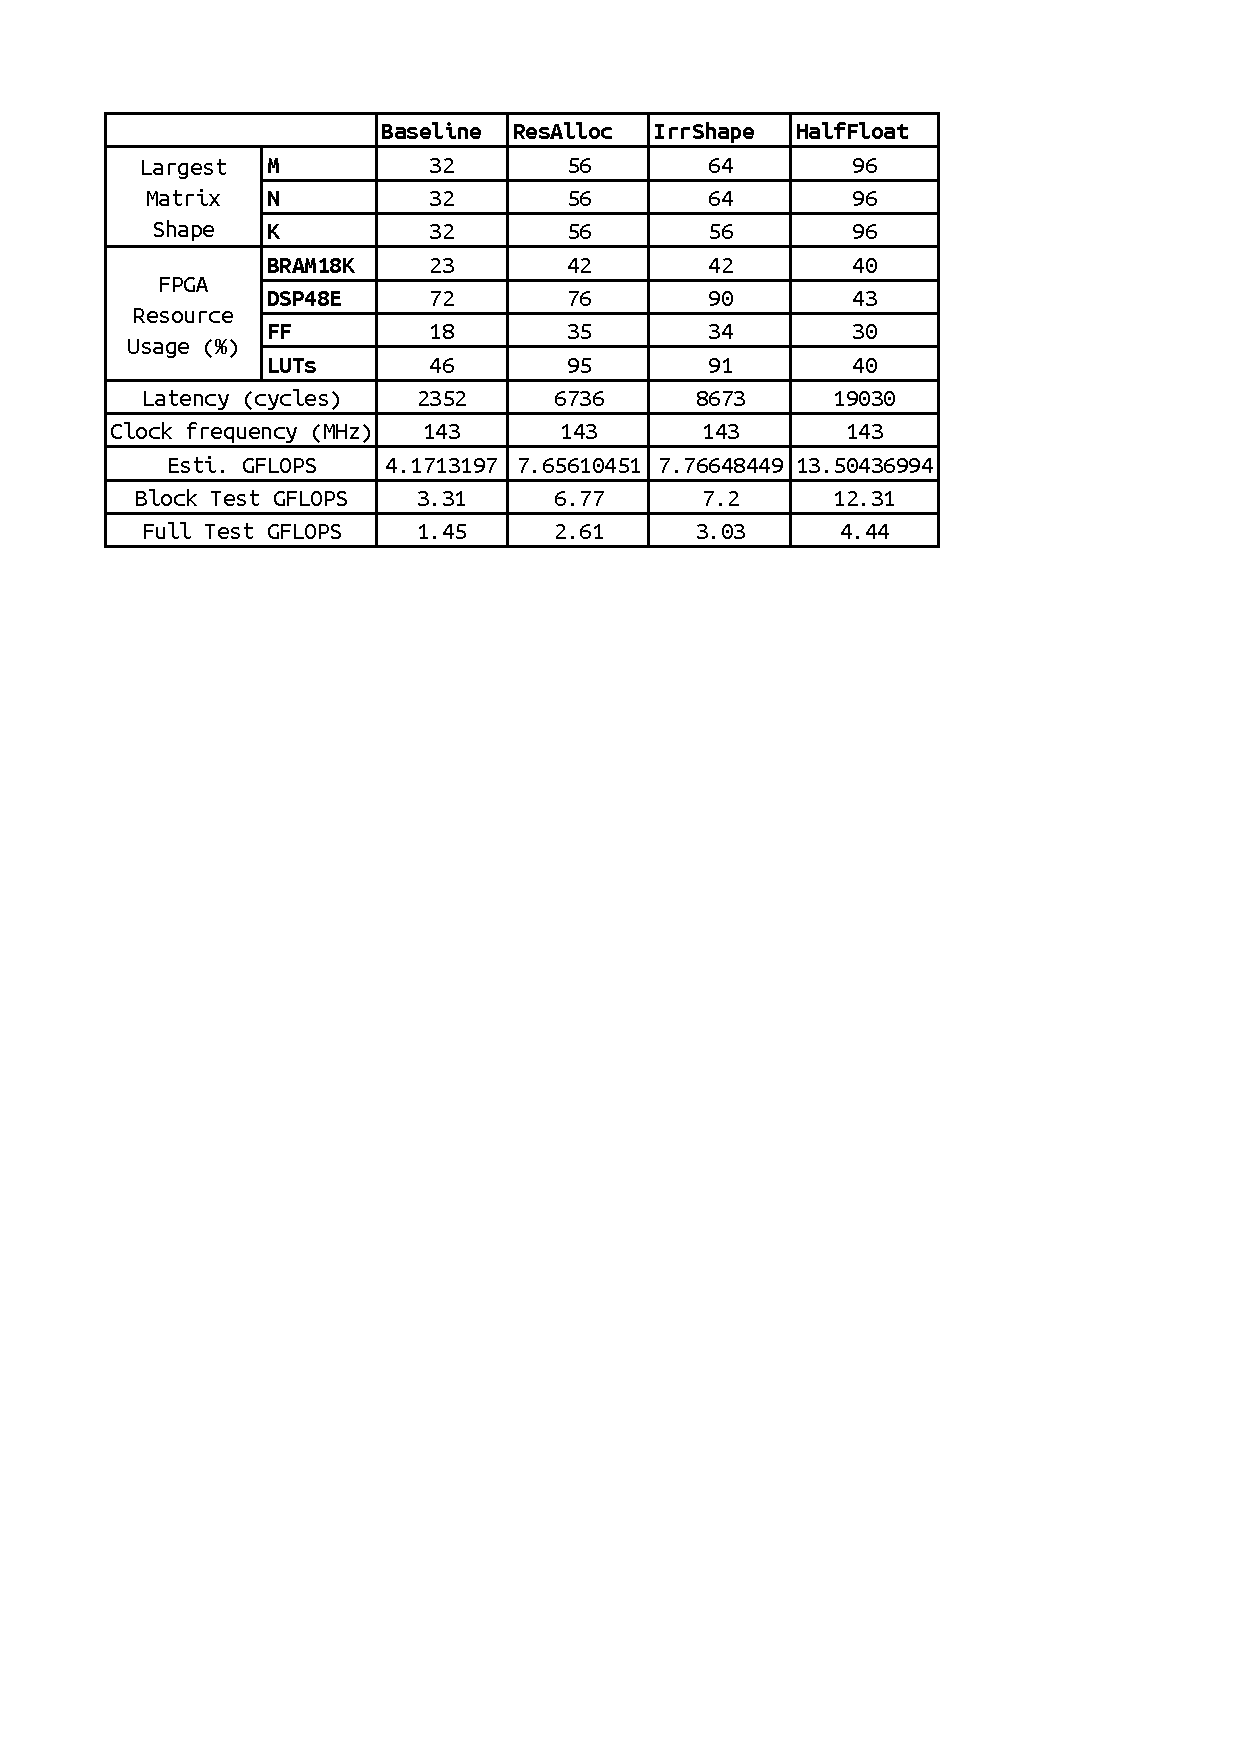
\includegraphics[width=0.9\textwidth]{assets/imgs/gemmopt.pdf}
\caption{GEMM优化策略对比结果}
\label{fig:gemmopt}
\end{figure}

根据\ref{subsec:gemmopt}节,得到如下四个版本实现:原始实现(Baseline)、资源分配优化(ResAlloc)、矩阵尺寸优化(IrrShape)以及半精度浮点数优化(HalfFloat)四个版本。本节选取四个版本的设计在最优参数配置下得到的实现作为对比样本,对比的项目包括:
\begin{enumerate}
\item 最大矩阵尺寸:根据目标版本,能得到的最大的矩阵尺寸;
\item FPGA资源利用:BRAM,DSP,LUT等指标所占用的百分比;
\item 延迟与时钟频率:时钟频率选用能综合得到的最快的时钟频率;
\item 预测性能与实际性能:用GFLOPS作为性能指标;
\end{enumerate}

对比结果参见图\ref{fig:gemmopt}。可以发现最快的优化版本是使用半精度浮点数优化的版本,GFLOPS与矩阵块的大小密切相关。尽管资源分配优化与矩阵尺寸优化在$K$对应的矩阵块尺寸上一致,但因为$M$与$N$的不同造成性能上矩阵尺寸优化略优。此外,实际性能测试包含两个,一个是块测试,即单纯测试从CPU调用FPGA上GEMM操作的时间;另一个是完整测试,包含完整的GEMM算法,从矩阵拷贝数据到缓存中的时间也要计入。可以看出CPU端的计算确实比较影响最终的计算性能。

\subsection{OpenBLAS对比测试}

OpenBLAS是非常成熟的BLAS计算库,而且也是Caffe兼容的BLAS库之一,因此其在ARM CPU上的运行时间可以作为GEMM硬件加速比的计算基准。

\begin{figure}[!ht]
\centering	
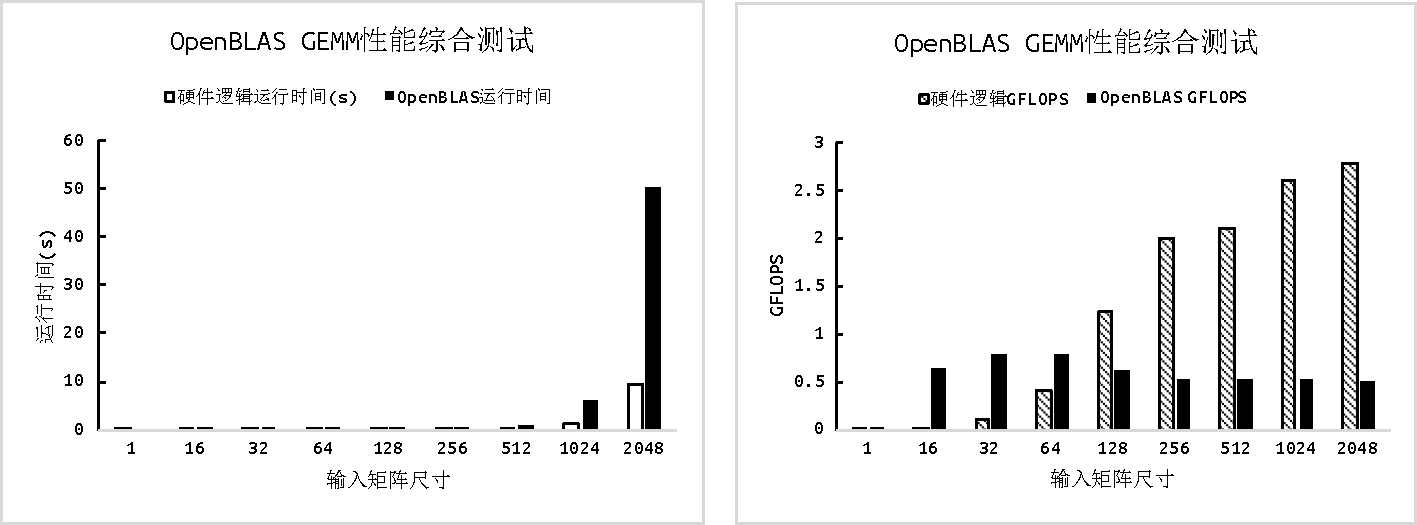
\includegraphics[width=\textwidth]{assets/imgs/gemmblas.pdf}
\caption{GEMM与OpenBLAS的性能对比}
\label{fig:gemmblas}
\end{figure}

这里测试使用的是GEMM在单精度浮点数精度下最快的版本(IrrShape)。与OpenBLAS在多种矩阵尺度下相比,GEMM硬件加速版本确实在小尺寸矩阵上速度很慢,但随着矩阵尺度大于128时,GEMM硬件加速比越来越大。最终测试结果显示GEMM的硬件加速版本是OpenBLAS的5.42倍。

\section{Caffe测试}

\subsection{单元测试}

Caffe的单元测试使用Google Test测试框架进行搭建,在功能性测试的基础上也加上简单的对性能的测试。

\subsection{网络性能测试}

\subsection{深度学习应用测试}

\subsubsection{MNIST}

\subsubsection{CIFAR-10}

